\documentclass{article}
\usepackage{algorithm}
\usepackage{algorithmic}
\usepackage[french]{babel}
\usepackage[utf8]{inputenc}

\usepackage{amsmath}
\usepackage{graphicx}
\usepackage[colorinlistoftodos]{todonotes}
\usepackage{url}
\usepackage{hyperref}
%pour la mise en page des tableaux
\usepackage{array}
\usepackage{tabularx}
\usepackage{setspace}
\usepackage{abstract}
\usepackage[T1]{fontenc}
\usepackage[top=2cm, bottom=2cm, left=2cm, right=2cm]{geometry}
\usepackage{subfig}
\usepackage{placeins}

\usepackage[utf8]{inputenc}
%régler l'espacement entre les lignes
\newcommand{\HRule}{\rule{\linewidth}{0.5mm}}

\title{rapport MOSIMA}
\author{j.jehyankaa }
\date{November 2018}

\usepackage{natbib}
\usepackage{graphicx}

\begin{document}

\begin{titlepage}
\begin{center}

% Upper part of the page. The '~' is needed because only works if a paragraph has started.

\includegraphics[width=0.35\textwidth]{./images/logo}~\\[1cm]

\textsc{\LARGE Sorbonne Université (Master ANDROIDE)}\\[1.5cm]

\textsc{\Large }\\[0.5cm]

% Title
\HRule \\[0.4cm]

{\huge \bfseries Projet MOSIMA\\
Reproduction partielle du modèle FIRE \\[0.4cm] }

\HRule \\[1.5cm]

% Author and supervisor
\begin{minipage}{0.4\textwidth}
\begin{flushleft} \large
\emph{Auteur:}\\
Jehyankaa \textsc{Jeyarajaratnam}\\
Binh Thanh \textsc{Luong}
\end{flushleft}
\end{minipage}
\begin{minipage}{0.4\textwidth}
\begin{flushright} \large
\emph{Référent:} \\
Jean-Daniel \textsc{Kant}
\end{flushright}
\end{minipage}

\vfill

% Bottom of the page
{\large \today}

\end{center}
\end{titlepage}
\tableofcontents
\newpage
\section{Étude préliminaire}
\subsection{Question 1.1}
 La problématique est la suivante : Représenter la notion de confiance et de réputation dans la société. On veut un modèle décentralisé et robuste permettant de représenter les relations de confiances entre deux types d’agents (consommateur et fournisseur) et la réputation de chacun de ces agents au sein de la société ainsi qu’au niveau individuel. Il faudra pouvoir distinguer la fiabilité d’une information en fonction de sa source. On veut également que ce modèle puisse s’adapter efficacement face à un SMA ouvert, c’est à dire face à un environnement et des agents dynamiques. 

Les auteurs proposent, pour cela, un modèle modulaire séparant la source des informations en quatre grandes catégories : IT (interactions directs), CR (valeurs certifiées fournies par le fournisseur), WR (témoignages), et RT (notes fournies par des agents ayant un lien avec le fournisseur). Les agents consommateurs, pourront donc adapter leur choix en fonction de ces différentes données et de l'importance qu'ils leur accordent.
D'autre part, plusieurs caractéristiques ont été mis en place pour justifier le dynamisme du modèle : La présence d’un agent n’est pas fixe. Des entrées et des sorties aléatoires se feront au cours de la simulation. Enfin, la situation individuelle d’un agent peut aussi changer entre deux cycles. Pour cela, les agent peuvent se déplacer et les performances des fournisseurs peuvent changer (parfois radicalement).

\subsection{Question 1.2}
Le modèle combine ces 4 composantes pour diversifier la source des informations et de ce fait la rendre plus réaliste (ce qui rend le modèle sera plus robuste). Parallèlement, le modèle distingue ces composantes afin de leur appliquer un poids adapté (ce qui est plus représentatif également).

\begin{figure}[h!]
\centering
\captionsetup{justification=centering}
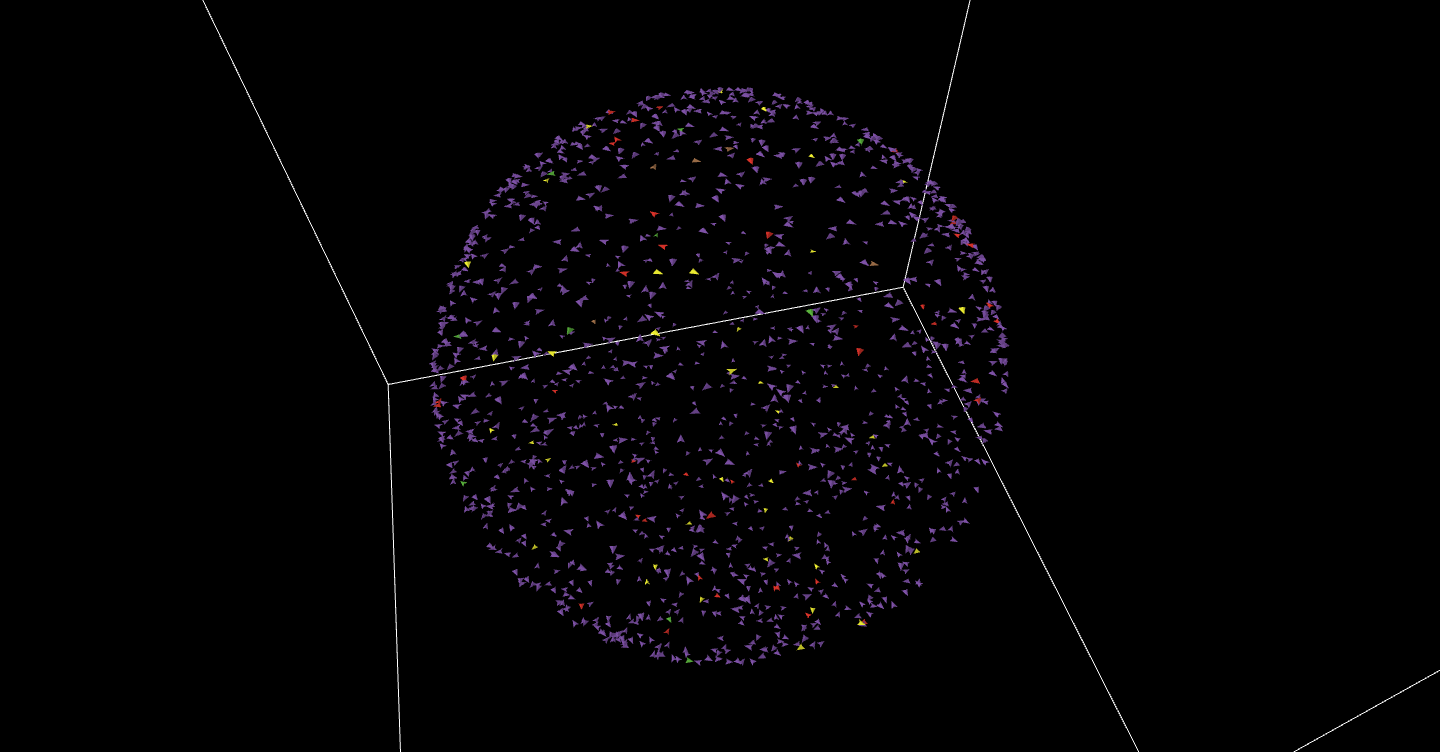
\includegraphics[width=0.5\textwidth]{images/world.png}
\caption{Spherical world \\(purple : consumers, green : good providers, yellow : ordinary providers, red : bad providers, brown : intermittent providers)}
\label{fig:universe}
\end{figure}


\section{Modèle avec composante IT seule (FIRE-IT)}
Toutes les figures représentées dans la suite du document peuvent être reproduites via les boutons correspondant et en lançant la simulation (\textit{GO})
\begin{figure}[H]
\centering
\captionsetup{justification=centering}
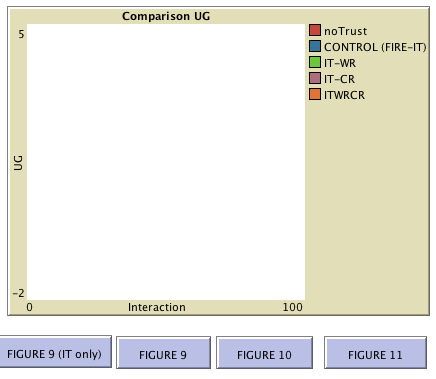
\includegraphics[width=0.5\textwidth]{images/captureInterface.png}
\caption{Interface}
\label{fig:interface}
\end{figure}
\subsection{Question 2.1.1}

\subsubsection{Structures}
Dans cette partie, nous détaillons les différentes principales structures de notre programme.
\label{sec:structures} 
\begin{itemize}
    \item \texttt{Rate} définit une note donnée. Elle est représentée sous la forme d'une liste telle que [a,b,i,v] où a est l'id du consommateur, b celui du fournisseur, i le temps d'enregistrement (tick) et v est la valeur de la note. Nous avons décidé de supprimer le terme c car il n'intervenait pas dans les calculs.
    \item \texttt{Consommateur}. L'agent consommateur possède les attributs suivants : un identifiant unique (automatique en NetLogo), un rayon d'opération (déterminé pour obtenir un voisinage spécifique), un niveau d'activité (aléatoire dans l'intervalle précisé dans l'article), une liste de \textit{Rates}, un modèle de confiance (parmi NoTrust, IT, ITWR, ITCR et ITWRCR) et deux listes hasTrustValue et noTrustValue. Ces deux listes permettent, à chaque tick, de trier les fournisseurs "connus" et inconnus. 

    \item \texttt{ProviderAgent}. L'agent fournisseur, quant à lui, possède également un identifiant et un rayon d'opération, mais aussi un type, un niveau de performance qui en découle. Le rayon d'opération, quelque soit le type d'agent, est déterminé arbitrairement. Ce choix est donc détaillé dans la partie \hyperref[sec:hypotheses]{Hypothèses}.
    
    \item \texttt{providerType} est une structure de type énumérations définie telle que : \newline
	\{\newline \quad good ([PL\_GOOD, PL\_PERFECT], 1.0), \newline \quad ordinary ([PL\_OK, PL\_GOOD], 2.0), \newline \quad bad ([PL\_WORST, PL\_OK], 2.0), \newline \quad intermittent (None, None) \newline	\}


\end{itemize}

\subsubsection{Algorithmes}
L'intégralité des algorithmes implémentés pour simuler le modèle FIRE-IT est présentée et détaillée ci-dessous. 
\textit{Remarque : À partir de l'algorithme 3, les pseudo-codes correspondent à des algorithmes conçus spécifiquement pour la partie IT seulement. Ils sont donc simplifiés car il s'agissait des bases mais assez complets pour la gestion du composant IT. Les méthodes ont été généralisées par la suite. Elles seront donc décrites dans les sections suivantes.}
\newline
Tous les agents dans cette environnement sont placés de manière aléatoire sur la surface de la sphère selon la distribution normale. Chaque agent possède des coordonnées cartésiennes satisfaisant l'équation de la sphère :

\[ x^2 + y^2 + z^2 = R^2 \]

\textit{R} étant le rayon fixé de la sphère et le centre est placé à l'origine O (0, 0, 0).
En partant de ces positions aléatoires, nous initialisons les agents de la manière suivante :

\begin{algorithm}[H]
\caption{Setup}
\begin{algorithmic}

\FORALL{consumersGroup c} 
\STATE create Nc consumers (c, random position)
\ENDFOR 
\STATE create NPB providers (type = bad , random position)
\STATE create NPO providers (type = ordinary , random position)
\STATE create NPG providers (type = good , random position)
\STATE create NPI providers (type = intermittent , random position)
\STATE setPerformances
\end{algorithmic}
\end{algorithm}
	








Avec \texttt{setPerformances} étant l'attribution aléatoire pour chaque fournisseur d'un niveau de performance correspondant à son type. Le tirage aléatoire s'effectue dans un intervalle particulier. En effet, chaque type de fournisseur correspond à un intervalle de performance (sauf pour les intermittents) et à une déviation (\hyperref[sec:structures]{Voir structures}). Les fournisseurs de type intermittents représentent une exception. Leur niveau de performance n'est pas réglé à l'initialisation mais sera généré aléatoirement lors des interactions.

Ensuite, la boucle principale est lancée (appelé à chaque \texttt{tick}). 

\begin{algorithm}[H]
\caption{Main}
\begin{algorithmic} 
\FORALL{Consumers}
\IF{random < activity-level} 
\STATE provider $\leftarrow$ search-provider
\STATE interact-with-provider
\ENDIF
\ENDFOR
\FORALL{Providers}
\STATE switch-behaviours
\ENDFOR
\FORALL{Consumers}
\STATE random-move
\ENDFOR
\STATE random-setup
\STATE delete-old-ratings
\STATE ticks ++
\IF{ticks > rounds-number} 
\STATE STOP
\ENDIF
\end{algorithmic}
\end{algorithm}

 
Les processus de sélection et l'interaction sont décrits ci-dessous tandis que les fonctions de dynamisme (random-move, random-setup et switch-behaviours) sont détaillées en fin de section.


\begin{algorithm}[H]
\caption{Search-provider IT}
\begin{algorithmic} 

\IF {t-model = NoTrust}
\STATE return get-random-provider
\ENDIF
\IF {t-model = IT}
\STATE search-list $\leftarrow$ nearby-providers
\FORALL {provider p in search-list}
\IF {get-rates-for (p) = $\emptyset$}
\STATE noTrustValue $\leftarrow$ p
\ELSE
\STATE hasTrustValue $\leftarrow$ p
\ENDIF
\ENDFOR
\IF{has-trust-value = $\emptyset$}
\RETURN select random provider
\ENDIF
\IF{no-trust-value = $\emptyset$}
\RETURN select best provider
\ENDIF
\STATE bestP $\leftarrow$ select-best-provider ()
\STATE $ER_{a1}$ $\leftarrow$ getTI (bestP)

\STATE $ER_{a2}$ $\leftarrow$ mean average-performance
\COMMENT {Average performance is determined considering the types of every provider in HasTrustValue $\cup$ NoTrustValue}


\STATE T $\leftarrow$ $\frac{T}{1.5}$

\STATE $p_{a1} \leftarrow \frac{\exp{\frac{ER_{a1}}{T}}}{\exp{\frac{ER_{a1}}{T}}+ \exp{\frac{ER_{a2}}{T}}}$

\IF {(random (0,1 ) < $p_{a1}$}
\STATE return bestP
\ELSE
\STATE return selectRandomProvider()
\ENDIF
\ENDIF
\end{algorithmic}
\end{algorithm}




La valeur initiale de T (la température déterminant le biais du choix entre les deux actions - dilemme de Boltzmann) ainsi que sa fonction de décroissance a été déterminée arbitrairement. L'opération initiale consistait à diviser T par une valeur à chaque sélection mais cela sera modifié ensuite (voir \hyperref[sec:temperature]{partie Hypothèses}). 

Parmi les fournisseurs de la liste \textit{hasTrustValue}, on tire le meilleur selon l'algorithme \textit{selectBestProvider}.

\begin{algorithm}[H]
\caption{Select Best Provider}
\begin{algorithmic}

\STATE bestV $\leftarrow$ Integer.MIN
\STATE bestP $\leftarrow$ None
\FORALL{p in hasTrustValue}
\STATE trustValue $\leftarrow$ getITTrustValue(p)
\IF{trustValue> bestV}
\STATE bestV $\leftarrow$ trustValue
\STATE bestP $\leftarrow$ p
\ENDIF
\ENDFOR

\RETURN bestP
\end{algorithmic} 
\end{algorithm}


Les "valeurs de confiances" (trust values) et la fiabilité de celles-ci (reliability) sont déterminées, pour le moment, comme ceci :

\begin{algorithm}[H]
\caption{get IT Trust Value}
\begin{algorithmic} 
\STATE valueSum $\leftarrow$ 0
\STATE weightSum $\leftarrow$ 0
\FORALL{r in R(a,b,c)}
\STATE weight $\leftarrow$ $\frac{\exp{ (-1*this.tick-r[i]) }}{\lambda}$

\STATE weightSum $\leftarrow$ weightSum + weight
\STATE valueSum $\leftarrow$ valueSum + weight * r[v]
\ENDFOR
\RETURN $\frac{somme}{weightSum}$
\end{algorithmic}
\end{algorithm}
\begin{algorithm}[H]
\caption{get IT reliability}
\begin{algorithmic} 
\STATE pd $\leftarrow$ 0
\STATE weightSum $\leftarrow$ 0
\FORALL{r in R(a,b,c)}
\STATE weight $\leftarrow$ $\frac{\exp{ (-1*this.tick-r[i]) }}{\lambda}$
\STATE weightSum $\leftarrow$ weightSum + weight
\STATE pd $\leftarrow$ pd + weight * |r[v] - TI|
\ENDFOR
\STATE pd $\leftarrow$ 1 - $\frac{pd}{2 * weightSum}$
\STATE pr $\leftarrow$ 1 - $\exp{-1 * gamma * weightSum}$
\RETURN pd * pr
\end{algorithmic}
\end{algorithm}
	
Il faut noter que la fiabilité ne sera pas utilisée pour cette partie car IT est la seule composante présente.

Une fois le fournisseur choisi, l'interaction se déroule :
\begin{algorithm}[H]
\caption{Interact-with (Provider p)}

\begin{algorithmic}
\STATE ug $\leftarrow$ getUG (p.type)

\IF{consumer out of provider's radius}
\STATE ug $\leftarrow$ ug*alpha*distance
\ENDIF
\STATE add-ug-to-list (t-model)
\STATE v $\leftarrow$ $\frac{ug}{10}$
\STATE self.ratings $\leftarrow$ self.ratings $\cup$ \{new Rate (self,provider, tick, v)\}

\end{algorithmic}
\end{algorithm}
L'UG est tirée suivant une distribution normale dont la moyenne est le niveau de performance de l'agent et l'écart-type correspondant à son type.
Dans le cas où le consommateur se trouverait hors du rayon d'opération du fournisseur, l'article nous décrit que l'UG décroît linéairement en fonction de ce facteur. Toutefois, il n'y a pas plus de précisions à ce sujet. Il a donc fallu émettre quelques hypothèses que l'on décrit dans la \hyperref[sec:hypotheses]{partie 8}.

À la fin de chaque tour, les bases de données locales (listes de notes stockées) sont mises à jour afin de ne garder que les H notes les plus récentes :

\begin{algorithm}[H]
\caption{Delete Old Ratings}
\begin{algorithmic} 
\STATE sort self.ratings by i in decreasing order
\STATE self.ratings $\leftarrow$ self.ratings[:H]
\end{algorithmic}
\end{algorithm}

Enfin, toutes les méthodes (\texttt{algo 4-6}) représentant le dynamisme du monde (et donc qui permettent de simuler les effets d'un système multi-agents ouvert), ont également été implémentées. Aucune d'entre elles n'intervient dans le cadre de ce projet mais il est possible de les activer séparément grâce aux switchs présents sur l'interface. (dynamism-move pour les déplacements des agents, dynamism-behaviours pour les changement de comportement des fournisseurs et dynamism-setup pour les entrées-sorties d'agents)
\begin{algorithm}[H]
\caption{Random Move}

\begin{algorithmic}

\IF{(type = provider \& random < pPLC) or (type = consumer \& random < pCLC)}
\STATE borne $\leftarrow$ $\frac{\pi}{20} $
\STATE $\delta\phi$ $\leftarrow$ random(-borne, borne)
\STATE $\delta\theta$ $\leftarrow$ random(-borne, borne)
\STATE r,$\theta$,$\phi$ $\leftarrow$ get-polar (x,y,z)
\STATE $\theta \leftarrow \theta + \delta\theta$
\STATE $\phi \leftarrow \phi + \delta\phi$
\STATE x,y,z $\leftarrow$ get-cartesian(r,$\theta$,$\phi$)
\STATE agent.moveTo(x,y,z)
\STATE agent.setNeighbours()
\ENDIF
\end{algorithmic}


\end{algorithm}
 
L'article décrit qu'un agent peut se déplacer en ajoutant à $\theta$ et à $\phi$ un angle appartenant à [-$\frac{\pi}{20}$,$\frac{\pi}{20}$]. Or, en Netlogo, un agent est décrit par ses coordonnées cartésiennes. Il nous faut donc passer par les coordonnées polaires pour réaliser les changements de locations. Ces conversions entre coordonnées cartésiennes et polaires sont décrites dans la partie \hyperref[sec:hypotheses]{Hypothèses et Formules}.
\begin{algorithm}[H]
\caption{Random Setup}
\begin{algorithmic}
\STATE n $\leftarrow$ random (0, $p_{CPC}$ * consumersCount) 
\STATE delete n consumers
\STATE add n consumers
\STATE n $\leftarrow$ random (0, $p_{PPC}$ * providersCount) 
\STATE delete n providers
\STATE add n providers
\end{algorithmic}

\end{algorithm}
\begin{algorithm}[H]
\caption{Switch behaviours}
\begin{algorithmic}
\IF {random < $p_{\mu C}$}
\STATE $\delta\mu \leftarrow$ random(-M,M)
\STATE newPerformance $\leftarrow$ oldPerformance + $\delta\mu$
\ENDIF
\IF {random < $p_{ProfileSwitch}$}
\STATE setNewProfile
\ENDIF
\end{algorithmic}

\end{algorithm}


\subsection{Question 2.1.2}
La procédure d'initialisation des agents a été expliquée dans la partie précédente. 
Les paramètres suivants ont été affichés sur l'interface afin de pouvoir les modifier manuellement : Nc(nombre de consommateurs par groupe), nombres de fournisseurs par types, rounds-number(durée de la simulation), H(taille de la liste des notes par agent), initT (Valeur initiale de la température qui détermine la probabilité de choisir une action entre explorer et exploiter (dilemme de Boltzmann\cite{Dilemme}).

\begin{figure}[H]
\begin{center}
\begin{tabular}{|l|l|l|l|l|l|l|l|}
  \hline
  Nc & NPB & NPO & NPG & NPI & rounds-number & H & initT\\
  \hline
  500 & 45 & 40 & 10 & 5 & 500 & 10 & 1 \\
  \hline
\end{tabular}
\end{center}
\caption{Paramètres d'IT}
\end{figure}

Voici l'évolution des simulations jusqu'à l'obtention d'une figure similaire à la figure 9.
\begin{figure}[H]
   \begin{minipage}{0.48\textwidth}
     \centering
     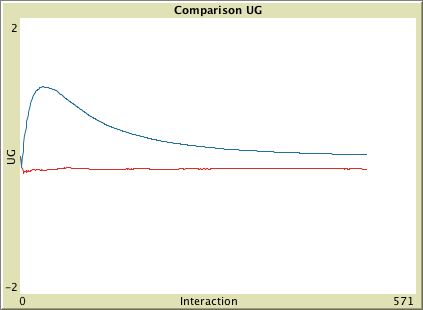
\includegraphics[width=.7\linewidth]{images/evolutionIT/IT1.png}
     \caption{IT-NoTrust : Plot 1}\label{Fig:Data1}
   \end{minipage}\hfill
   \begin{minipage}{0.48\textwidth}
     \centering
     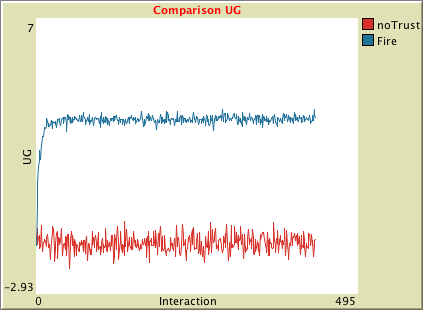
\includegraphics[width=.7\linewidth]{images/evolutionIT/IT2.png}
     \caption{IT-NoTrust : Plot 2}\label{Fig:Data2}
   \end{minipage}
\end{figure}

Le plot 1 représente la toute première courbe obtenue après l'implémentation des algorithmes. Nous pensions d'abord que la baisse après une trentaine d'itérations était dû à un H trop petit (taille de mémoire insuffisante). Finalement, nous avons obtenu le plot 2 après avoir inclus la prise en compte de la distance lors du calcul de $ER_{a2}$ (résultat attendu pour explore\cite{Dilemme}). En effet, la moyenne des niveaux de performances de tous les fournisseurs était retournée mais la distance à laquelle se trouvaient ces derniers n'était pas incluse dans le calcul. Il faut préciser, ici, que nous avions supposé (à tort) qu'un agent consommateur prenait la liste de tous les fournisseurs du monde avant sa sélection. A ce stade du projet (partie IT seule), nous n'avions pas remarqué qu'il ne prenait que ses voisins. Il arrivait donc que l'UG obtenue après une interaction soit très éloignée du $ER_{a2}$. Ceci a corrigé l'erreur du plot 1. 
\begin{figure}[H]
   \begin{minipage}{0.48\textwidth}
     \centering
     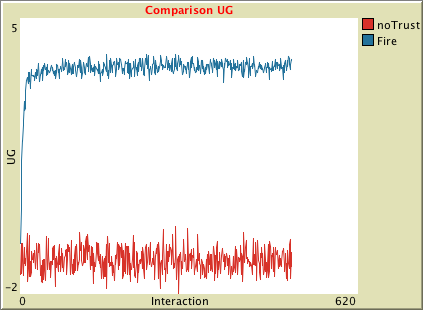
\includegraphics[width=.7\linewidth]{images/evolutionIT/IT3.png}
     \caption{IT-NoTrust : Plot 3}\label{Fig:Data1}
   \end{minipage}\hfill
   \begin{minipage}{0.48\textwidth}
     \centering
     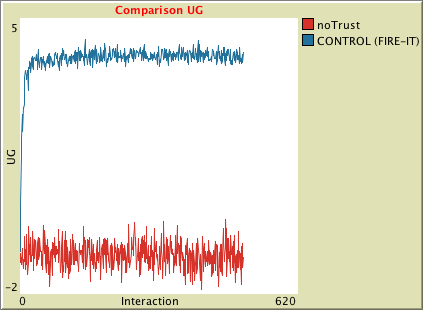
\includegraphics[width=.7\linewidth]{images/evolutionIT/IT4.png}
     \caption{IT-NoTrust : Plot 4}\label{Fig:Data2}
   \end{minipage}
\end{figure}

Ensuite, nous avons réussi à faire augmenter la moyenne en modifiant la variable T (température). Nous l'avons finalement initialisé à 1 puis diminué de 0.1\% à chaque interaction de l'agent.
\subsection{Question 2.1.3}
Finalement, après avoir corrigé les erreurs décrites ci-dessus (notamment la liste initiale pour la sélection des fournisseurs), la figure 9 est reproduite.

\begin{figure}[H]
\centering
\captionsetup{justification=centering}
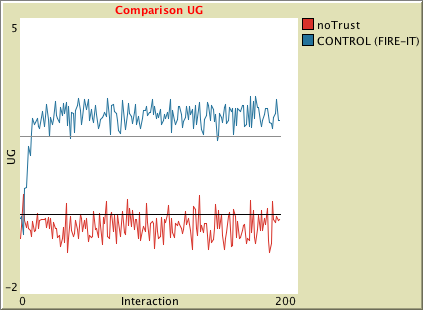
\includegraphics[width=0.3\textwidth]{images/evolutionIT/IT5.png}
\caption{Reproduction de la figure 9 (pour CONTROL = FIRE-IT)}
\label{fig:fig9}
\end{figure}

Le résultat est similaire à celui de l'article à la seule différence près que la courbe croît (et donc se stabilise) plus vite que celle d'origine. Ce phénomène est vient peut-être du fait que les agents ont tendance à passer à l'exploitation plus vite. Deux facteurs peuvent causer ceci : le rayon des agents est trop petit (pas assez de voisins) ou la température décroît trop vite. D'autre part, nous avons également remarqué une variabilité au niveau de la convergence de la courbe entre plusieurs simulations avec des paramètres identiques. Cette différence reste toutefois négligeable.
Pour que le résultat soit plus ressemblant à l'article, c'est-à-dire pour que la courbe soit plus lisse, il est possible de garder tous les UGs obtenue depuis le début de la simulation. Ainsi, on ne viderait pas les listes à chaque \texttt{tick} mais il nous paraissaît plus cohérent d'avoir une moyenne d'UGs obtenue sur les données d'une itération seulement.

\section{Modèle avec composantes IT et WR (FIRE-IT-WR)}
\subsection{Question 2.2.1}
Avec la composante WR, nous effectuons la recherche des témoignes. 2 paramètres sont introduits dans cette partie sont nBF (facteur de branchement) et nRL (seuil de longueur de référence). Lors de la sélection d'un fournisseur, le consommateur envoie une requête à nBF de ses voisins les plus susceptibles de connaître le fournisseur dont on cherche une valeur de confiance. La sélection parmi les voisins s'effectue avec la mesure de distance qui le sépare du fournisseur. Les agents ayant reçu cette requête renvoie, soit les notes du fournisseur s'ils ont effectivement eu une interaction avec, soit une liste de leurs voisins susceptibles de le connaître. Ainsi cette boucle s'itère jusqu'à ce que la longueur de la chaîne atteigne nRL ou jusqu'à ce que le consommateur ait trouvé nBF témoins (c'est à dire nBF agents ayant eu une interaction avec le fournisseur).

\begin{algorithm}[H]
\caption{WR-Evaluation}
\begin{algorithmic} 
\STATE chainLength $\leftarrow$ 0
\STATE witnessNb $\leftarrow$ 0
\STATE ratingsList $\leftarrow$ [ ]
\STATE acquaintances $\leftarrow$ [ ]
\WHILE{acquaintances.length < nbF}
\STATE acquaintances $\leftarrow$ likelyAcquaintances
\ENDWHILE
\WHILE{witnessNb < nBF and chain < nRL}
\STATE chain ++
\FORALL{Provider p in acquaintances}
\STATE acquaintances.remove(self)
\IF {matchingRatingsFound}
\STATE ratingsList $\leftarrow$ ratingList $\cup$ ratings
\STATE witnessNb ++
\ELSE
\STATE acquaintances $\leftarrow$ acquaintances $\cup$ listOFnewAcquaintances
\ENDIF
\ENDFOR
\ENDWHILE

\STATE RW $\leftarrow$ ratingsList
\STATE TV $\leftarrow$ getTrustValue (WR)
	
\end{algorithmic}
\end{algorithm}





Quand le consommateur reçoit les notes des témoins, il évalue ces notes et celles de sa base de données locale pour avoir une valeur de confiance avec l'ensemble des informations qu'il possède. Nous avons donc du modifier la méthode getTValue pour la rendre générique.

\begin{algorithm}[H]
\caption{get Trust Value}
\begin{algorithmic} 
\STATE t-value $\leftarrow$ 0
\STATE weightSum $\leftarrow$ 0
\STATE r-ab $\leftarrow$ $\empty$
\FORALL{k in every components of t-model}
    \STATE r-ab $\leftarrow$ get-rates-for b from component k
    \STATE tk $\leftarrow$ get-t-value-by-component r-ab
    \STATE reliability $\leftarrow$ get-reliability for component k
    \STATE w $\leftarrow$ get-component's coefficient * reliability
    \STATE t-value $\leftarrow$ t-value + component's weight * tk
    \STATE weight-sum $\leftarrow$ weight-sum + w
\ENDFOR
\STATE t-value $\leftarrow$ t-value / weight-sum
\RETURN t-value
\end{algorithmic}
\end{algorithm}

où getTValueByComponent correspond à :

\begin{algorithm}[H]
\caption{get Trust Value for b by Component k}
\begin{algorithmic} 
\STATE t-value $\leftarrow$ 0
\STATE weightSum $\leftarrow$ 0

\IF{k = IT}
\STATE r-ab $\leftarrow$ self.getRates(b)
\ENDIF
\IF{k = WR}
\STATE r-ab $\leftarrow$ wr-evaluation(b)
\ENDIF
\IF{k = CR}
\STATE r-ab $\leftarrow$ b.receivedRatings
\ENDIF

\FORALL{r in r-ab}
\STATE ug $\leftarrow$ r[v] * 10
\STATE ug $\leftarrow$ ug + $\delta$UG
\STATE v $\leftarrow$ ug / 10
\STATE weight $\leftarrow$ $\frac{\exp{ (-1*this.tick-r[i]) }}{\lambda}$
\STATE weightSum $\leftarrow$ weightSum + weight
\STATE t-value $\leftarrow$ t-value + weight * v
\ENDFOR
\STATE t-value $\leftarrow$ t-value / weightSum
\RETURN t-value
\end{algorithmic}
\end{algorithm}


$\delta$UG sera expliqué dans la partie 4.2.

La méthode getReliability a également été modifiée de la même manière.

\subsection{Question 2.2.2}
Nous avons du modifier quelques paramètres afin d'obtenir une simulation acceptable. Lorsque un groupe de consommateurs avec le composant WR (IT-WR ou IT-WR-CR) est présent, nous avons remarqué que le lancement était beaucoup trop lent. N'ayant pas pu régler ce problème dans les délais, nous devions diminuer soit le nombre de consommateurs par groupe (Nc) soit la longueur des chaînes de recherches de témoins (nRL). C'est finalement cette dernière qui a été diminuée. 

\subsection{Question 2.2.3}
\begin{figure}[H]
    \centering
    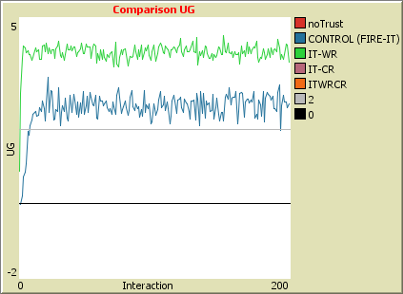
\includegraphics[width=0.8\textwidth]{images/ITvsITWR.png}
    \caption{Reproduction de la figure 9}
    \label{fig:itvswr}
\end{figure}

Comme expliqué ci-dessus, le temps d'exécution était très grand même après l'optimisation du code. Nous avons, entre autres, crée un attribut \texttt{neighbours} propre à chaque agents afin de ne pas lancer la recherche de voisins plusieurs fois. Malgré cet inconvénient, et le changement de paramètres liés, nous avons quand même un résultat assez convenable. \newline La présence du composant WR permet aux agents d'accéder à des informations concernant un fournisseur plus rapidement.
\section{Modèle avec composante IT, WR et CR (FIRE-IT-WR-CR)}
\subsection{Question 2.3.1}
Les lignes suivantes seront ajoutées à la fin de l'algorithme interact-with. Le fournisseur choisit la meilleure note parmi celles que le consommateur a enregistré. Il gardera donc toujours une note par interaction avec un consommateur différent mais il peut choisir la meilleure parmi ces interactions.
\begin{algorithm}[H]
\caption{Store certified reputation}

\begin{algorithmic}
\STATE allRatings $\leftarrow$ get-rates-for (provider)
\STATE bestRate $\leftarrow$ max(allRatings)
\STATE provider.receivedRatings $\leftarrow$ provider.receivedRatings $\cup$ bestRate

\end{algorithmic}
\end{algorithm}

Donc \texttt{get-rates(CR, p)} renvoie la liste \texttt{receivedRatings} (de taille H au maximum) du fournisseur p.

\subsection{Question 2.3.2}
Nous avons modifié le code afin que le système prenne un nouveau paramètre en compte : la différence de distance lorsqu'on a une note venant d'un autre consommateur (WR ou CR) car il y a des chances que ce dernier soit plus proche du fournisseur. Il faut donc ajuster la performance attendue en fonction de cette différence. Le calcul de celle-ci est décrit dans la partie \hyperref[sec:hypotheses]{Hypothèses}. Cette modification a été faite dès l'implémentation du composant WR.

\subsection{Question 2.3.3}
\begin{figure}[H]
   \begin{minipage}{0.48\textwidth}
     \centering
     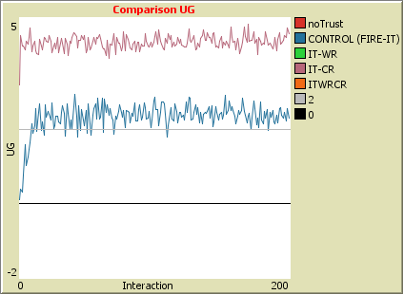
\includegraphics[width=.7\linewidth]{images/ITvsITCR.png}
     \caption{Reproduction figure 10 (ITWR - ITCR)}\label{Fig:Data1}
   \end{minipage}\hfill
   \begin{minipage}{0.48\textwidth}
     \centering
     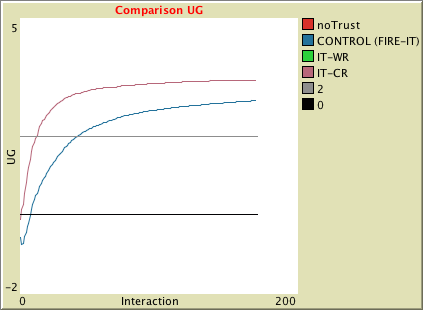
\includegraphics[width=.7\linewidth]{images/ITvsITCR2.png}
     \caption{IT-ITCR sans vider les UGs}\label{Fig:Data2}
   \end{minipage}
\end{figure}

\begin{figure}[H]
\centering
\captionsetup{justification=centering}
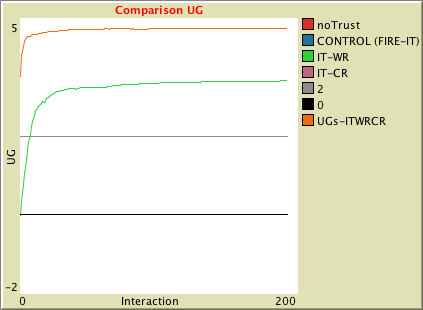
\includegraphics[width=0.4\linewidth]{images/ITWRvsITWRCR.png}
\caption{Reproduction figure 11 (ITWR - ITWRCR)}
\label{fig:fig11}
\end{figure}

Afin de rendre le résultat plus lisible, nous avons gardé les listes des UGs sans les vider pour la reproduction de la figure 11.
Nous remarquons que la présence du composant CR donne une UG quasiment égale à celle que nous apportait le composant WR tout en étant beaucoup plus rapide. La recherche de témoins prenait beaucoup plus temps à s'exécuter, ce qui est compréhensible étant donné le grand nombre d'agents. Le modèle ITCR est aussi beaucoup plus performant dès les premières interactions, ce qui est logique car il y a 100 fournisseurs pour 500 consommateurs. Un fournisseur a plus de chances d'effectuer sa première interaction plus vite qu'un consommateur.
Sur la figure 11, nous remarquons que le modèle ITWRCR converge plus vite que ITWR. Nous supposons que, grâce à une collecte rapide des informations (via CR), les agents connaissent plus vite leur environnement et se mettent en mode 'exploitation' plus rapidement.

\subsection{Question 2.3.4}
\begin{figure}[H]
\centering
\captionsetup{justification=centering}
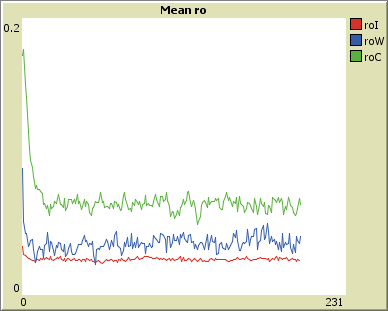
\includegraphics[width=0.8\textwidth]{images/ROs.png}
\label{fig:ROs}
\end{figure}
Nous remarquons que les trois courbes diminuent rapidement. Cependant les fiabilités de IT restent très basses et stables pendant toute la simulation.
D'autre part, la courbe des fiabilité de la composante CR reste au dessus de celle de WR qui est, elle même, au dessus de celle de IT. L'explication pour ce phénomène est le poids des composantes : $W_I$=2, $W_W$=1 et $W_C$=0.5.
Nous remarquons que l'évolution des courbes reflète symétriquement celle des courbes des UGs. Il faut rappeler que les choix entre exploration et exploitation étaient les facteurs principaux des apparences de ces courbes. En effet, les probabilités de choisir une action ou une autre sont à peu près égales au début ($p_{a1}$=$p_{a2}$=0.5). Puis la probabilité de choisir l'exploitation plutôt que l'exploration augmente. Cette évolution correspond à la quantité d'informations qu'un agent possède sur son monde. Nous pouvons donc supposer que la tendance à exploiter ces informations est à l'origine de la diminution des valeurs de fiabilité.
\section{Analyse de sensibilité du modèle FIRE-IT-WR-CR}
Dans cette partie, nous étudions l'influence des paramères sur le modèle
\subsection{Question 2.4.1}
Tout d'abord nous allons étudier l'impact du nombre de consommateurs. Nous avons fixé les paramètres comme décrit le tableau ci-dessous :

\begin{table}[H]
    \centering
    \begin{tabular}{|c|c|c|c|c|c|c|}
    \hline
         NP: [NPG,NPO,NPI,NPB] & H & [nBF,nRL] & initialTemperature & rounds-number & initialNc & incrementNc\\ \hline
         [10,40,5,45] & 10 & [2,5] & 500 & 200 & 50 & 50\\\hline
    \end{tabular}
    \caption{Experimental setup}
    \label{tab:Experimental setup1}
\end{table}

Pour chacune des 10 valeurs différentes de Nc variant de 50 à 500, nous avons lancé l'expérience pour un nombre d'itération de 200. Les résultats obtenus sont regroupés dans la figure \ref{fig:UGNc} suivante :

\begin{figure}[H]
\centering
\captionsetup{justification=centering}
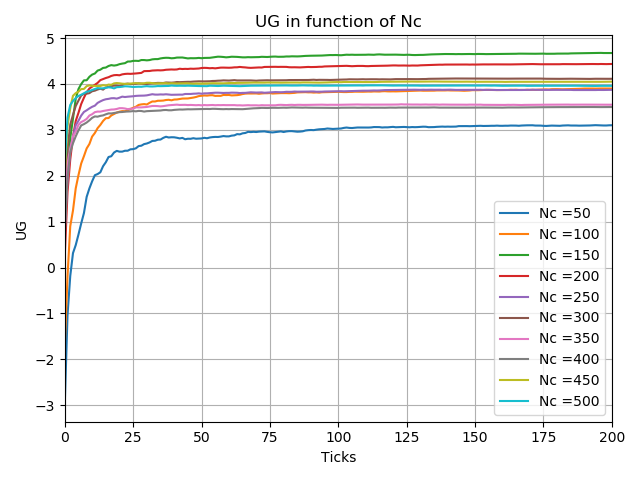
\includegraphics[width=0.8\textwidth]{images/UGinfunctionNc.png}
\caption{UG in function of Nc}
\label{fig:UGNc}
\end{figure}

Nous pouvons constater que les courbes pour les Nc variant entre 100 et 500 sont très proches et indistinguables. La courbe pour Nc = 50 est plus faible que les autres. Une explication pour ce phénomène est que la densité des agents sur la sphère est assez faible et leur rayon de communication est petit. Lors d'une recherche de témoin, l'agent ne peut pas avoir assez d'information sur un fournisseur à cause du manque de voisins voire aucun voisin donc il devra choisir un fournisseur aléatoire. C'est donc aussi la raison pour laquelle les valeurs de Nc medianes (150, 200) donnent des courbes plus puissantes que les autres car l'agent a suffisamment des voisins pour brancher assez proche à un fournisseur. Le fait d'avoir plusieurs voisins dans son rayon de communication ne garantie pas l'obtention des informations sur un agent. Un agent ne cherche que parmi ses voisins ceux qui sont les plus proche du fournisseur qui ont potentiellement jamais en contact avec le fournisseur.

\subsection{Question 2.4.2}
Dans cette question, nous avons analysé l'influence des poids des composants WR et CR. Nous avons utilisé les valeurs par défaut de FIRE \cite{firemodel} (Wi = 2, Ww = 1, Wc= 0.5) pour déterminer l'intervalle de définition ainsi que le nombre de réplications. Nous avons donc choisi de faire varier les variables Ww et Wc dans l'intervalle [0.5,2]. La valeur 2 est prise comme une borne supérieure car aucune composante ne peut donner la valeur de fiabilité plus forte que la confiance en soi qui est très approché du monde réel. Voici les paramètres par défaut de l'expérience :

\begin{table}[H]
    \centering
    \begin{tabular}{|c|c|c|c|c|c|}
    \hline
         NP: [NPG,NPO,NPI,NPB] & H & [nBF,nRL] & initialTemperature & rounds-number & Nc\\ \hline
         [10,40,5,45] & 10 & [2,5] & 500 & 200 & 250\\\hline
    \end{tabular}
    \caption{Experimental setup}
    \label{tab:Experimental setup2}
\end{table}
Le résultat obtenu est la figure \ref{fig:UGwwwc} ci-dessous :
\begin{figure}[H]
\centering
\captionsetup{justification=centering}
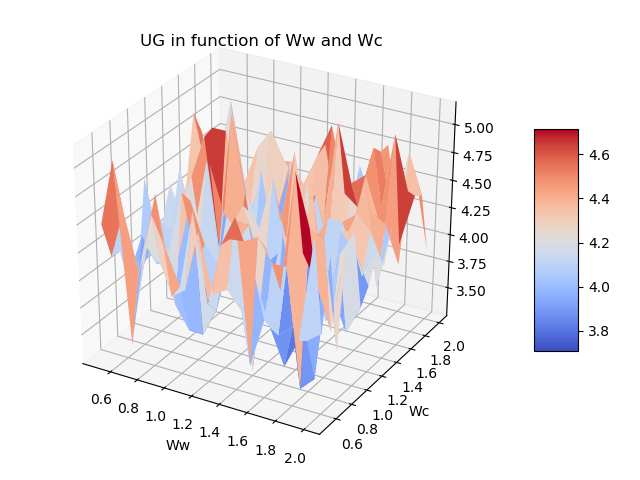
\includegraphics[width=0.8\textwidth]{images/3Dwwwc.png}
\caption{UG in function of Wc and Wc}
\label{fig:UGwwwc}
\end{figure}
Nous pouvons évidemment constater que le coefficient Wc implique l'utilité du modèle : plus ce poids est important, plus l'utilité globale est grande. Lors de mise à jour de mémoire, l'agent fournisseur ne garde que ses meilleures notes obtenues au cours du temps. Quand il donne ses notes aux consommateurs, cela affecte fortement le choix des consommateurs.

\subsection{Question 2.4.3}
Nous allons maintenant calculer la distributions des UGS aux consommateurs après un lancement. Dans la figure \ref{fig:distribution} ce-dessous, nous voyons la moyenne des UGs distribuées à chaque consommateur.
\begin{figure}[H]
    \centering
    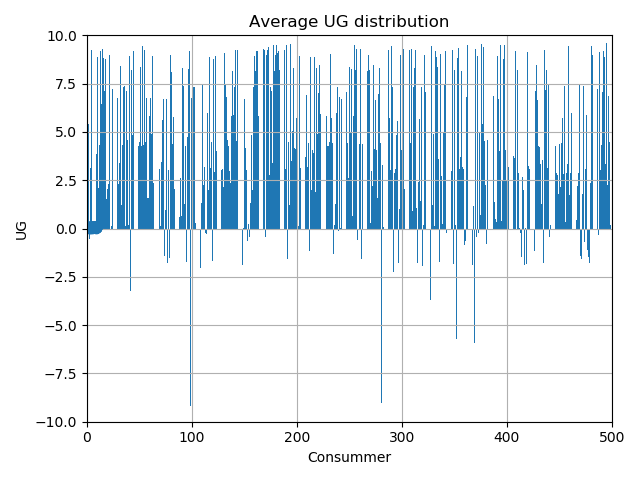
\includegraphics[width=0.8\textwidth]{images/Distribution.png}
    \caption{Distribution des UGs des clients}
    \label{fig:distribution}
\end{figure}
La distribution des UGs est globalement uniforme.

\subsection{Question 2.4.4}
En respectant le nombre de fournisseurs est à 100, nous avons fait varier les paramères NPB, NBO, NB pour observer l'impact de ses paramètres. Nous avons effectué 6 configurations dont une est les paramètres par défaut afin de pouvoir juger l'importance de ses paramètres. Les paramètres fixés sont décrits dans le tableau ci-dessous :
\begin{table}[H]
    \centering
    \begin{tabular}{|c|c|c|c|c|}
    \hline
         H & [nBF,nRL] & initialTemperature & rounds-number & Nc\\ \hline
         10 &[2,5] & 500 & 200 &250\\\hline
    \end{tabular}
    \caption{Experimental setup}
    \label{tab:Experimental setup3}
\end{table}
Le résultat obtenu est le suivant :
\begin{figure}[H]
    \centering
    \subfloat[Average UG]{{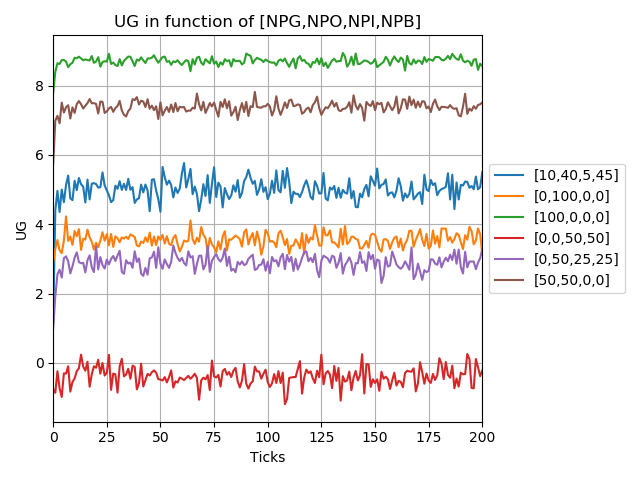
\includegraphics[width=0.45\linewidth]{images/UGinfunctionNp.png} }}%
    \qquad
    \subfloat[Standard-deviation]{{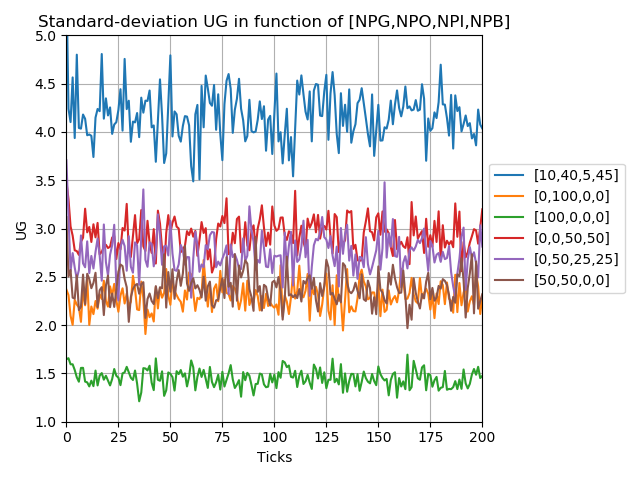
\includegraphics[width=0.45\linewidth]{images/UGsdinfunctionNp.png} }}%
    \caption{UG and its standard-deviation in function of Np}%
    \label{fig:UGNp}%
\end{figure}

Le schéma montre que NPG joue un rôle très important. Bien évidemment s'il existe seulement de bon fournisseurs, les consommateurs obtiennent des UGs très grandes ainsi que l'écart type est faible. Cependant, si les fournisseurs sont divers (paramètres par défaut), l'écart type grand. Dans ce modèle, la distance est un facteur aussi important car UG décroît en fonction de la distance entre 2 agents.

\section{Extension}
Nous avons décidé d'implémenter l'extension 2 en introduisant des agents menteurs. Ces mensonges interviennent dans les deux composantes suivantes : WR et CR. Les consommateurs peuvent fournir de fausses notes lorsque le fournisseur leur demande une certification ou quand un autre consommateur les contacte pour un témoignage. Pour ce dernier, nous avions pensé à deux alternatives : inventer une interaction qui n'a jamais eu lieu et envoyer la fausse note ou se baser sur l'ensemble de notes existant pour le modifier. Cette dernière a été choisie car elle permet de garder une certaine logique dans les fausses notes : qu'ils proviennent de CR ou WR, il s'agit toujours d'un écart par rapport à une vraie note. Ce genre de notes biaisées nous semblait être le plus réaliste et le plus commun.
Nous avons posé un intervalle [-0.75,0.75] dans lequel une valeur $\epsilon$ sera tirée aléatoirement. Ainsi \[NewRate = OldRate + \epsilon\].
\subsection{Résutats}
Contrairement à nos attentes, les agents s'en sortent plutôt bien. Ce qui montre que le modèle FIRE est robuste aux mensonges.

\begin{figure}[H]
    \begin{minipage}{0.3\textwidth}
     \centering
     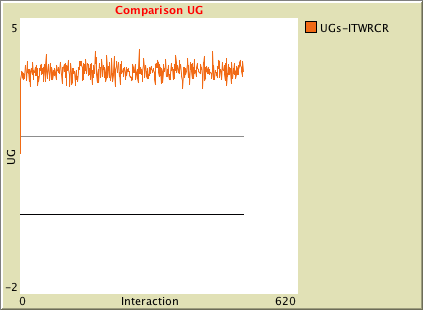
\includegraphics[width=.6\linewidth]{images/evolutionLiars/20.png}
     \caption{20\% de menteurs}\label{Fig:Data2}
   \end{minipage}
   \begin{minipage}{0.3\textwidth}
     \centering
     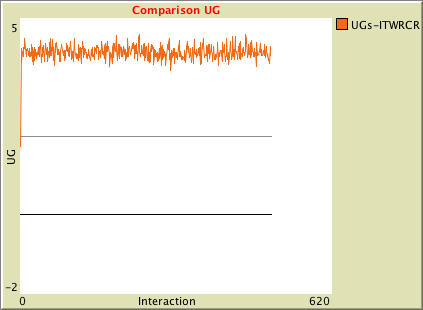
\includegraphics[width=.6\linewidth]{images/evolutionLiars/50.png}
     \caption{50\% de menteurs}\label{Fig:Data1}
   \end{minipage}
   \begin{minipage}{0.3\textwidth}
     \centering
     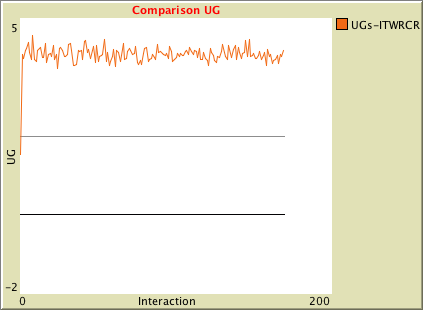
\includegraphics[width=.6\linewidth]{images/evolutionLiars/80.png}
     \caption{80\% de menteurs}\label{Fig:Data2}
   \end{minipage}
\end{figure}





\section{Nosedive}
Afin d'adapter et étendre le modèle pour simuler l'épisode \textit{Nosedive} de \texttt{BlackMirror}, nous pourrions rajouter des notes pour les consommateurs : n'importe quel agent (fournisseur ou consommateur) pourrait noter un consommateur selon l'attitude qu'il a eu lors d'une interaction donné (pas forcément à but lucratif). Après une interaction avec un fournisseur choisi grâce à la méthode recherche de témoins, le consommateur pourrait noter le témoin (en se basant sur la différence entre son témoignage et la performance reçue). Ces modifications nécessitent l'inclusion d'attitudes chez les agents. Il faudrait donc définir des groupes d'agents ayant un comportement défini. Similairement au type des fournisseurs, il y aurait de bons agents, des mauvais ou des imprévisibles. Cet attribut déterminerait leur caractère. 
Il faudrait ensuite restreindre certaines actions à un ensemble d'agents. C'est-à-dire que seulement les agents ayant une note supérieure à un certain seuil pourrait effectuer ces actions. 
Enfin, comme la notion de besoin n'existe pas chez les agents en Netlogo, nous devrions nous arranger pour que l'agent agisse stratégiquement pour obtenir ce dont il a besoin (i.e modifier temporairement son caractère dans le but de récolter de bonnes notes).  


\section{Hypothèses et formules}
\label{sec:hypotheses}
\subsection{Notation}
L'article ne montre pas explicitement la manière d'attribuer une note à une performance dont l'agent gagne une certaine utilité. Toutefois les intervalles de ces deux valeurs sont précisés : $UG \in [-10;10]$ et $v \in [-1;1]$. Nous avons opté pour la manière la plus simple de noter, $v = UG/10$ mais il est possible de biaiser cette notation (selon des agents dont le comportement serait différent par exemple). Cette alternative peut être intéressante si l'application du modèle le requiert. 

Enfin, étant donné que les performances sont tirées selon une distribution normale autour des moyennes, il se peut qu'elles dépassent [-10;10]. Dans ces cas, le programme remet les valeurs dans l'intervalle.

\subsection{Rayon d'opération}
L'article ne décrit pas la manière de choisir le rayon d'opération. Nous avons donc posé deux intervalles dans lesquelles les agents tirent une valeur aléatoirement pour définir leur rayon d'opération. Pour plus de réalisme, nous avons décidé d'attribuer, en général, un rayon plus grand pour les fournisseurs que pour les consommateurs. En effet, l'article compare le rayon d'opération d'un fournisseur à la distance entre deux grandes régions du monde (pays, continent...) et celui d'un consommateur à un voisinage proche. Cette même logique a été appliqué à notre modèle.
On a donc $C_{R_o} \in [0.1;0.4]$ et $P_{R_o} \in [0.5;1]$


\subsection{Régression de l'utilité en fonction de la distance}
Lorsqu'un agent consommateur ne se situe pas dans le rayon d'opération d'un fournisseur, la performance qui résulte de l'interaction en sera affecté. Par conséquent l'utilité sera dégradée (linéairement). En l'absence de données, nous avons dû déterminé le facteur de régression pour cette fonction. Le facteur :\[ \alpha = \frac{1}{c*D_{MAX}} \]. 

\emph{c} : ce coefficient permet de mesurer l'impact qu'aura la distance sur l'UG. Plus c sera grand moins une performance sera modifiée et plus c sera petit plus la distance qui sépare un consommateur (hors de portée) d'un fournisseur impactera l'UG. Dans notre cadre, nous le fixons à 100.

$D_{MAX}$ : la distance maximum qui peut séparer deux agents situé sur une sphère de rayon R. Nous considérons qu'il s'agit de la moitié de la circonférence du grand cercle c'est-à-dire \[ D_{MAX} = \pi * R \].

Ainsi, si l'utilité sera affecté de la manière suivante  \[ UG = UG - ( |UG|*(d-r_o)*\alpha\]. où $(d-r_o)$ représente la distance qui sépare le consommateur de rayon d'opération du fournisseur.

Cette régression devra être prise en compte lorsqu'une information concernant un fournisseur vient d'une tierce personne. En effet quand le consommateur \texttt{a} demande au consommateur \texttt{c} la note qu'il a mis pour le fournisseur {b}, il faut prendre en compte, en plus de la différence de temps $\delta$t(comme décrit dans l'article), la différence de distance. Nous cherchons donc à estimer l'\texttt{UG1} que l'agent \texttt{a1} tirera de l'interaction en connaissant l'\texttt{UG2} que l'agent \texttt{a2} a eu de cette façon : \[ UG1 = UG2 + \delta UG\].
avec
\[ \delta UG = \alpha*(d_2-d_1) \]
Étant donné que l'écart $\delta$UG ajouté dépend de la différence de distance entre a1 et a2, dans le cas d'une interaction directe (a1=a2), on aura bien $\delta$UG = 0.


\subsection{Calcul de distance}
Pour déterminer la distance qui sépare deux agents, nous avons décidé d'utiliser la distance du grand cercle plutôt qu'une distance euclidienne car plus représentative du monde réel (sphérique).

\begin{figure}[h!]
\centering
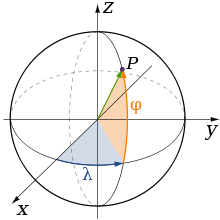
\includegraphics[scale=0.5]{images/great-circle-distance-img.png}
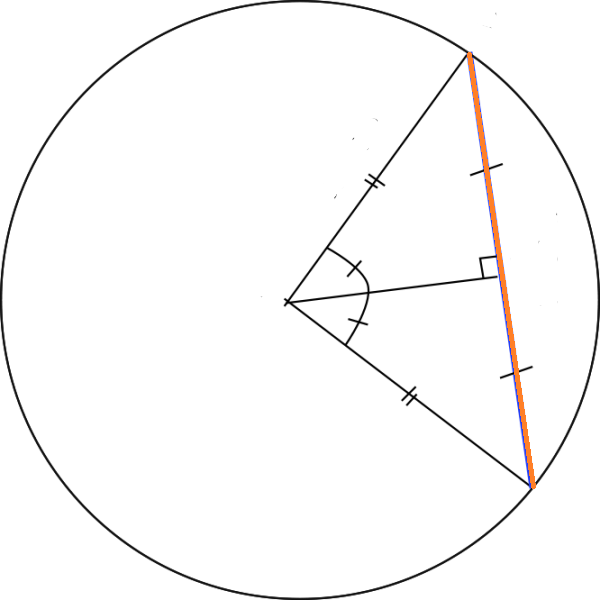
\includegraphics[scale=0.2]{images/distance-euclidienne.png}
\caption{Distance du grand cercle - Distance euclidienne}
\label{fig:Distance du grand cercle}
\end{figure}

Pour ce faire, nous avons eu besoin de convertir les coordonnées (cartésiennes par défaut) selon les formules suivantes \cite{conversion} : 

Cartésiennes -> Polaires
\[
   r = \sqrt{x^2 +y^2 + z^2} 
  \].
   \[
  \theta = \arccos\frac{z}{r}
    \].
     \[
  \phi = \arctan\frac{y}{x}
\].

Polaires -> Cartésiennes
\[
   x = r\sin{\theta}\cos{\phi}
  \].   
   \[
   y = r \sin{\theta}\sin{\phi}
   \]. 
    \[
   z = r\cos{\theta}
\].

La distance sera ensuite déterminée ainsi \cite{distance} :

\[ D = R\arcsin{\frac{d\sqrt{4R^2-d^2}}{2R^2}} \].
avec $ d^2 = (x_1-x_2)^2 + (y_1-y_2)^2 + (z_1-z_2)^2 $

\subsection{Température \cite{Dilemme}}
\label{sec:temperature}
La température est un facteur apparaissant dans le dilemme de Boltzmann mais dont la valeur dépend totalement de l'application.
Après de multiples changements et tests, elle a finalement été initialisé à 500 (le nombre d'interactions pour une simulation) et est décrementée à chaque tour.

\bibliographystyle{plain}
\bibliography{references}

\end{document}
